\documentclass[a4paper,11pt,oneside]{book}

\usepackage{amsmath}

\usepackage[T1]{fontenc}
\usepackage[utf8]{inputenc}

\usepackage{authblk}
\usepackage{float}% example bilder
\usepackage{array}

%\usepackage{pdfpages}
\usepackage{layout}

%---------- | < Dokument Einstellungen > | ----------
\title{Wechselrichter dreiphasig}
%\author{testAutor}

%---------- | < document > | ---------
\begin{document}
\pagestyle{plain}

\author[*]{Adrian Bucher}
\author[**]{Raphael Wirtz}
\author[***]{Pirmin Zimmermann}
%\author[1,2]{Pirmin Zimmermann\thanks{pirmin.zimmermann@stud.hslu.ch}}
\affil[*]{adrian.bucher@stud.hslu.ch}
\affil[**]{raphael.wirtz@stud.hslu.ch}
\affil[***]{pirmin.zimermann@stud.hslu.ch}

\renewcommand*{\Authsep}{\\}
\renewcommand*{\Authand}{\\}
\renewcommand\Authands{\\}

%---------- | < Titelblatt > | ----------
\thispagestyle{empty}
\begin{titlepage}	% noetig?
\begin{titlepage}
    \begin{center}
        \textbf{\huge{Hochschule Luzern}}\\
        \vspace{2mm}
        \large{Technik \& Architektur}\\
        \vspace{5mm}
    \end{center}

    \vspace{0mm}

    \begin{center}
        %\includegraphics[trim=0cm 4cm 0cm 0cm,clip=true, width=1\linewidth]{../common/figure/Titelblatt.jpg}
        \addcontentsline{lof}{figure}{Titelbild}
    \end{center} 

    \vspace{2mm}

    \begin{center}
        \rule{\textwidth}{2pt}
    \end{center}

    \begin{center}
      \textbf{\huge{EAT Testat}}\\
        \vspace{2mm}
        \Large{\makeatletter \@title  \makeatother}\\
        \vspace{2mm}
        \large{Laborversuch}
    \end{center}

    \begin{center}
        \rule{\textwidth}{2pt}
    \end{center}


    \begin{minipage}{0.7\textwidth}
    	\vspace{0pt}
        \begin{flushleft}
            Verfasst von:\\
            %\texttt{\textbackslash \@author}
            \large{\makeatletter \@author \makeatother}\\
            \vspace{4mm}
        \end{flushleft}
    \end{minipage}
    \begin{minipage}{0.3\textwidth}
    \vspace{0pt}
        \begin{flushright}
            Betreut von:\\
            \large{Prof. Dr. Adrian Omlin}
            \vspace{1mm}
        \end{flushright}
    \end{minipage}

	\vspace*{\fill}
    \begin{center}
        Horw, \today
    \end{center}

\end{titlepage}
\clearpage
\end{titlepage}
\clearpage 

\frontmatter	%römische Nummerierung aktivieren

%----- | < Inhaltsverzeichnis > | -----
%--- | TOC | ---
\usetocstyle{allwithdot}
%\settocfeature{}
\dominitoc
\tableofcontents
\adjustmtc
\addtocontents{toc}{~\hfill\textbf{Seite}\par}
\clearpage
%--- | LOF | ---
\dominilof
\listoffigures
\adjustmtc
\mtcaddchapter
\nomlfpagenumbers
\addcontentsline{toc}{chapter}{Abbildungsverzeichnis}
\addtocontents{lof}{~\hfill\textbf{Seite}\par}
\clearpage
%--- | LOF | ---
\dominilot
\listoftables
\adjustmtc
\addcontentsline{toc}{chapter}{Tabellenverzeichnis}
\addtocontents{lot}{~\hfill\textbf{Seite}\par}
\mtcaddchapter
\clearpage

%Symbolverzeichniss ????$$

%\chapter{Abkürzungen}
%\input{acronyms}
%\clearpage

\chapter{Aufgabenstellung}

%---------- | < Mainmatter > | ----------
\mainmatter		%arabische Nummerierung aktivieren
\chapter{Einrichtung}
\begin{itemize}  
\item Dreiphasiger Wechselrichter mit programmierbaren Pulsmustern
(Abbildung \ref{fig:einreichting_DreiphasigerWechselrichter})
\item Gleichrichter ABB DCS500 zur dc-seitigen Speisung des Wechselrichters
(Abbildung \ref{fig:einrichtung_Gleichrichter})
\item ASM Maschinensatz mit 5.5 kW
(Abbildung \ref{fig:einrichtung_ASM})
\item Drehmomentmesswelle
(Abbildung \ref{fig:einrichtung_Drehmomentswelle})
\item GM als Bremse
(Abbildung \ref{fig:einrichtung_Gleichstrommotor})
\end{itemize}

\begin{figure}[h]
	\centering
	\begin{subfigure}[b]{0.45\textwidth}
		\includegraphics[width=\textwidth]{images/ASM.JPG}
		\caption{ASM}
        \label{fig:einrichtung_ASM}
	\end{subfigure}
	\hfill
	\begin{subfigure}[b]{0.45\textwidth}
		\includegraphics[width=\textwidth]{images/Gleichstrommotor.JPG}
		\caption{Gleichstrommotor}
		\label{fig:einrichtung_Gleichstrommotor}
	\end{subfigure}
\end{figure}

\begin{figure}[h]
\centering
\ContinuedFloat % Nummerierung der zuvorkommenden figure vortführen (a,b,...)
\subcaptionbox{Drehmomentswelle\label{fig:einrichtung_Drehmomentswelle}}
  [.3\linewidth]{\includegraphics[width=5cm,angle=-90]{images/Drehmomentswelle.JPG}}
  \hfill
\subcaptionbox{Dreiphasiger Wechselrichter programmierbar\label{fig:einreichting_DreiphasigerWechselrichter}}
  [.3\linewidth]{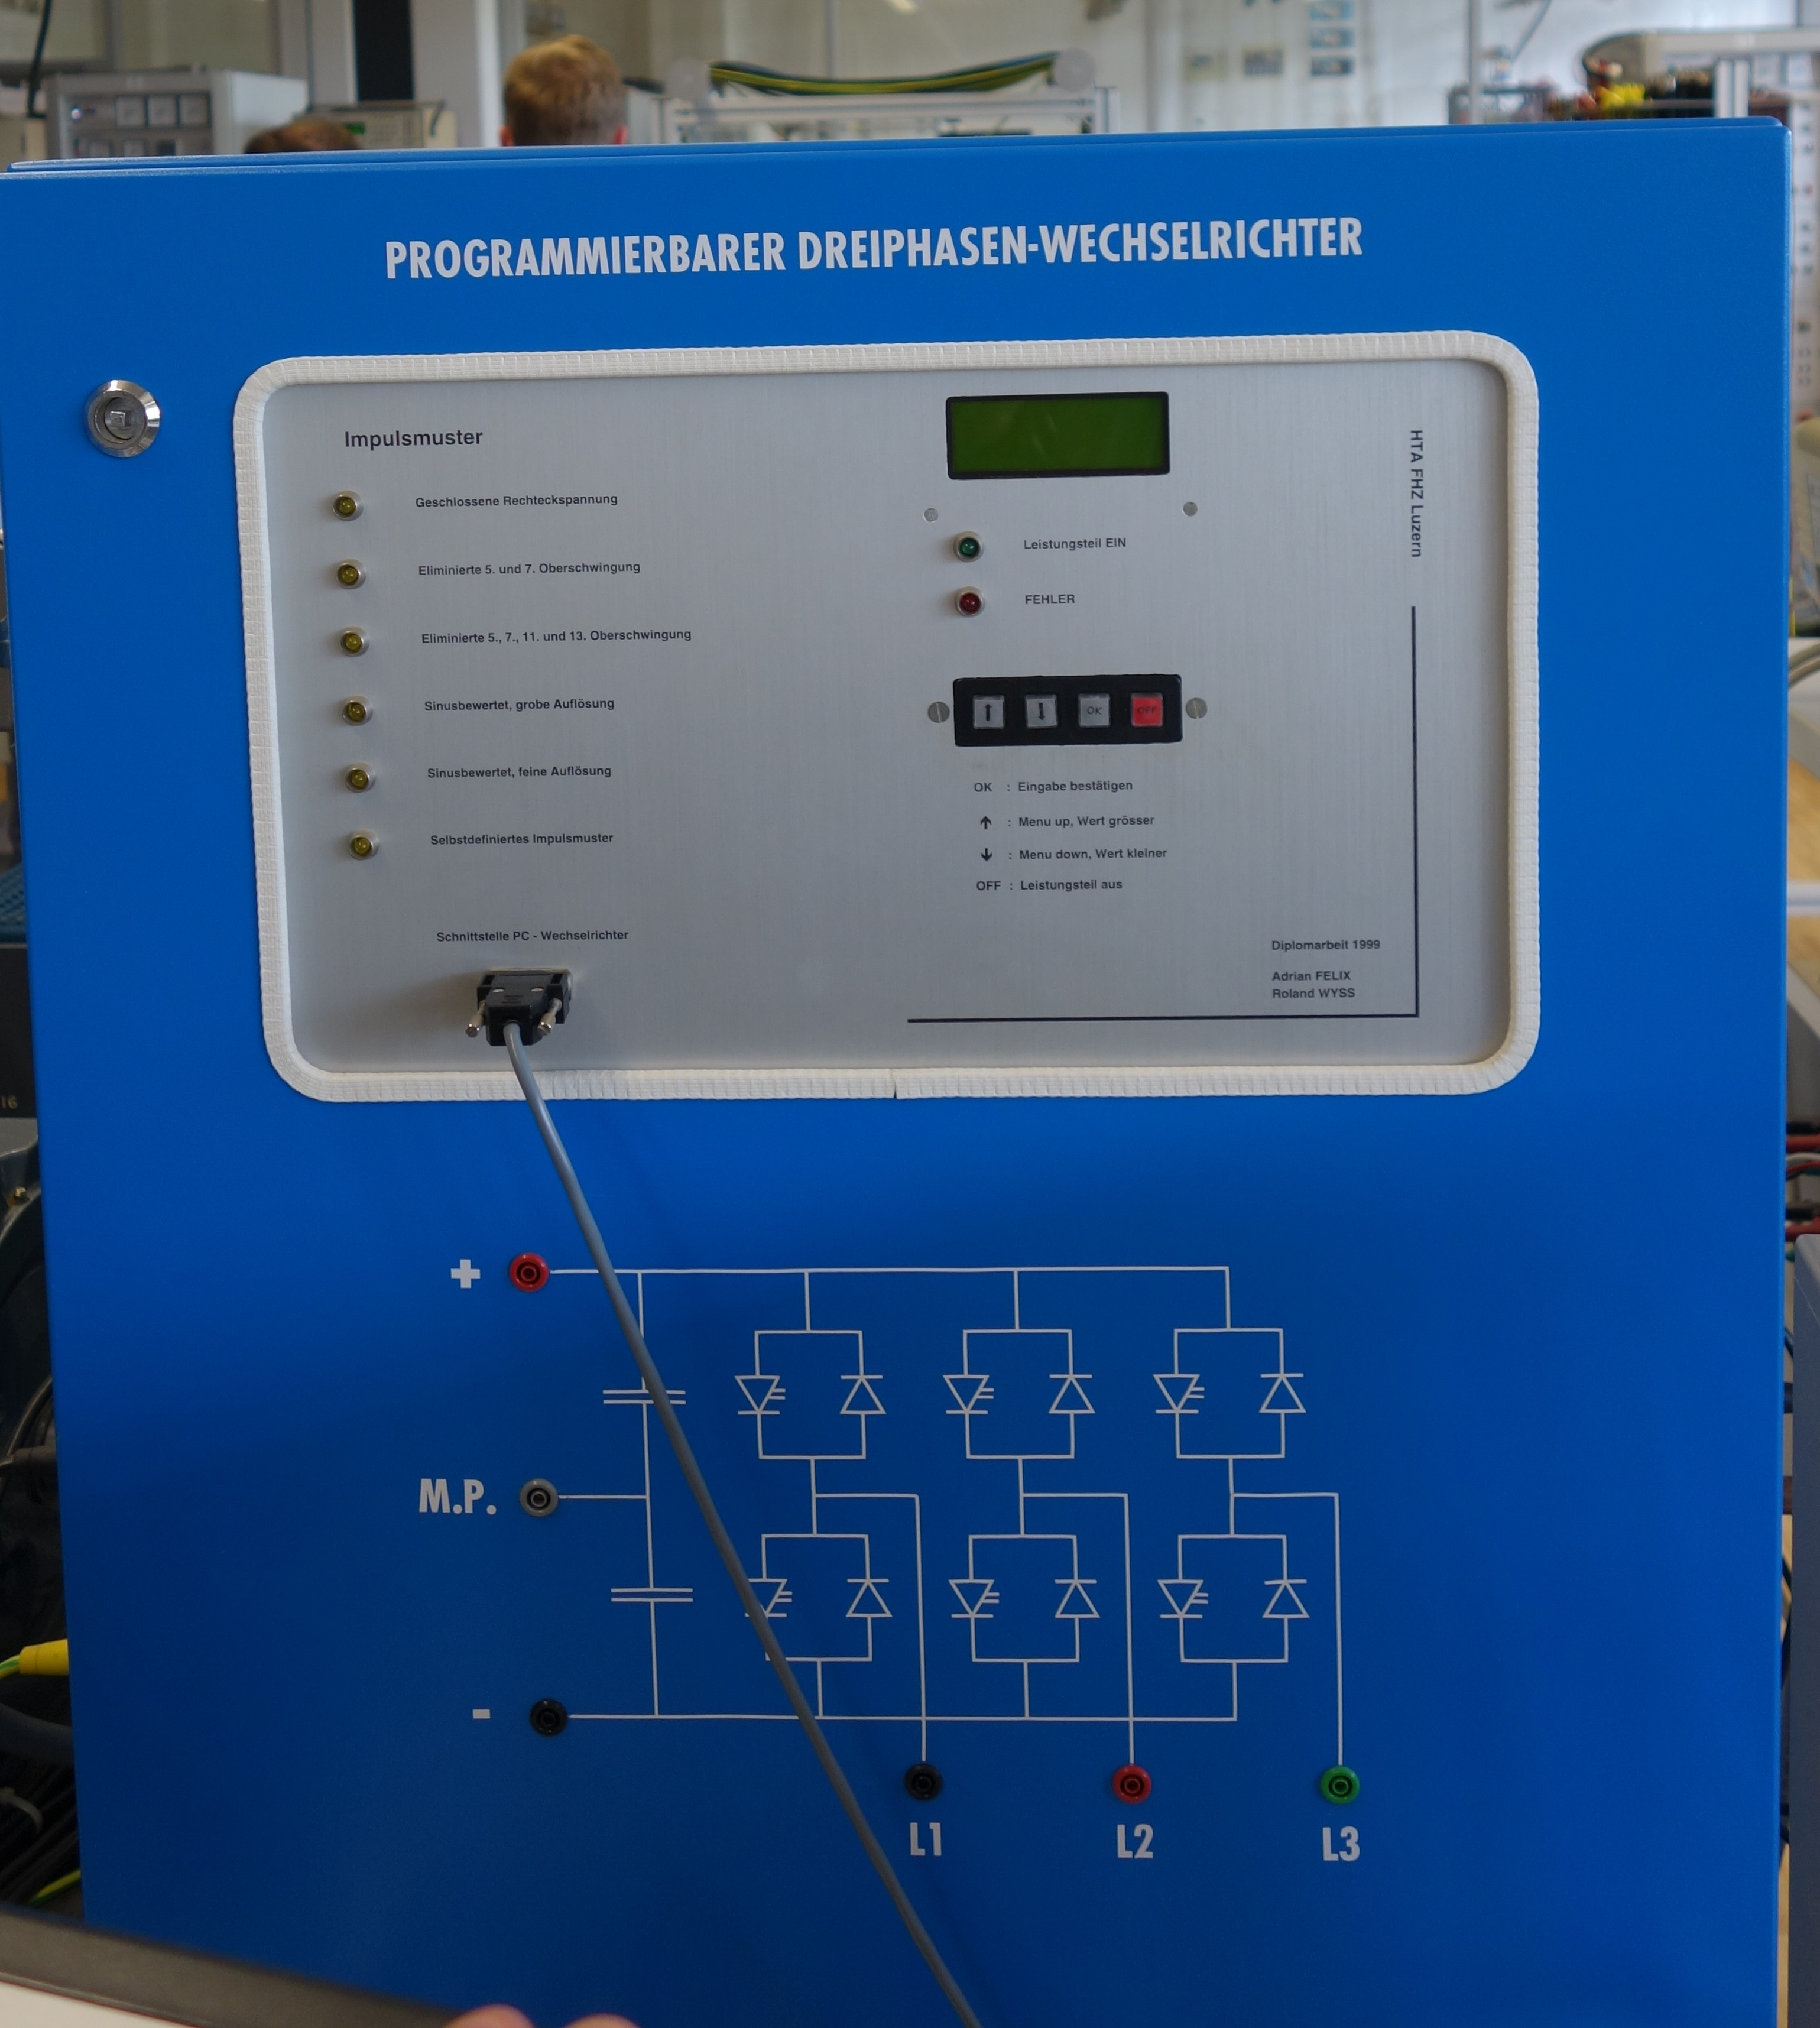
\includegraphics[height=5cm]{images/DreiphasigerWechselrichter_programmierbar.JPG}}
  \hfill
  \subcaptionbox{Gleichrichter\label{fig:einrichtung_Gleichrichter}}
  [.3\linewidth]{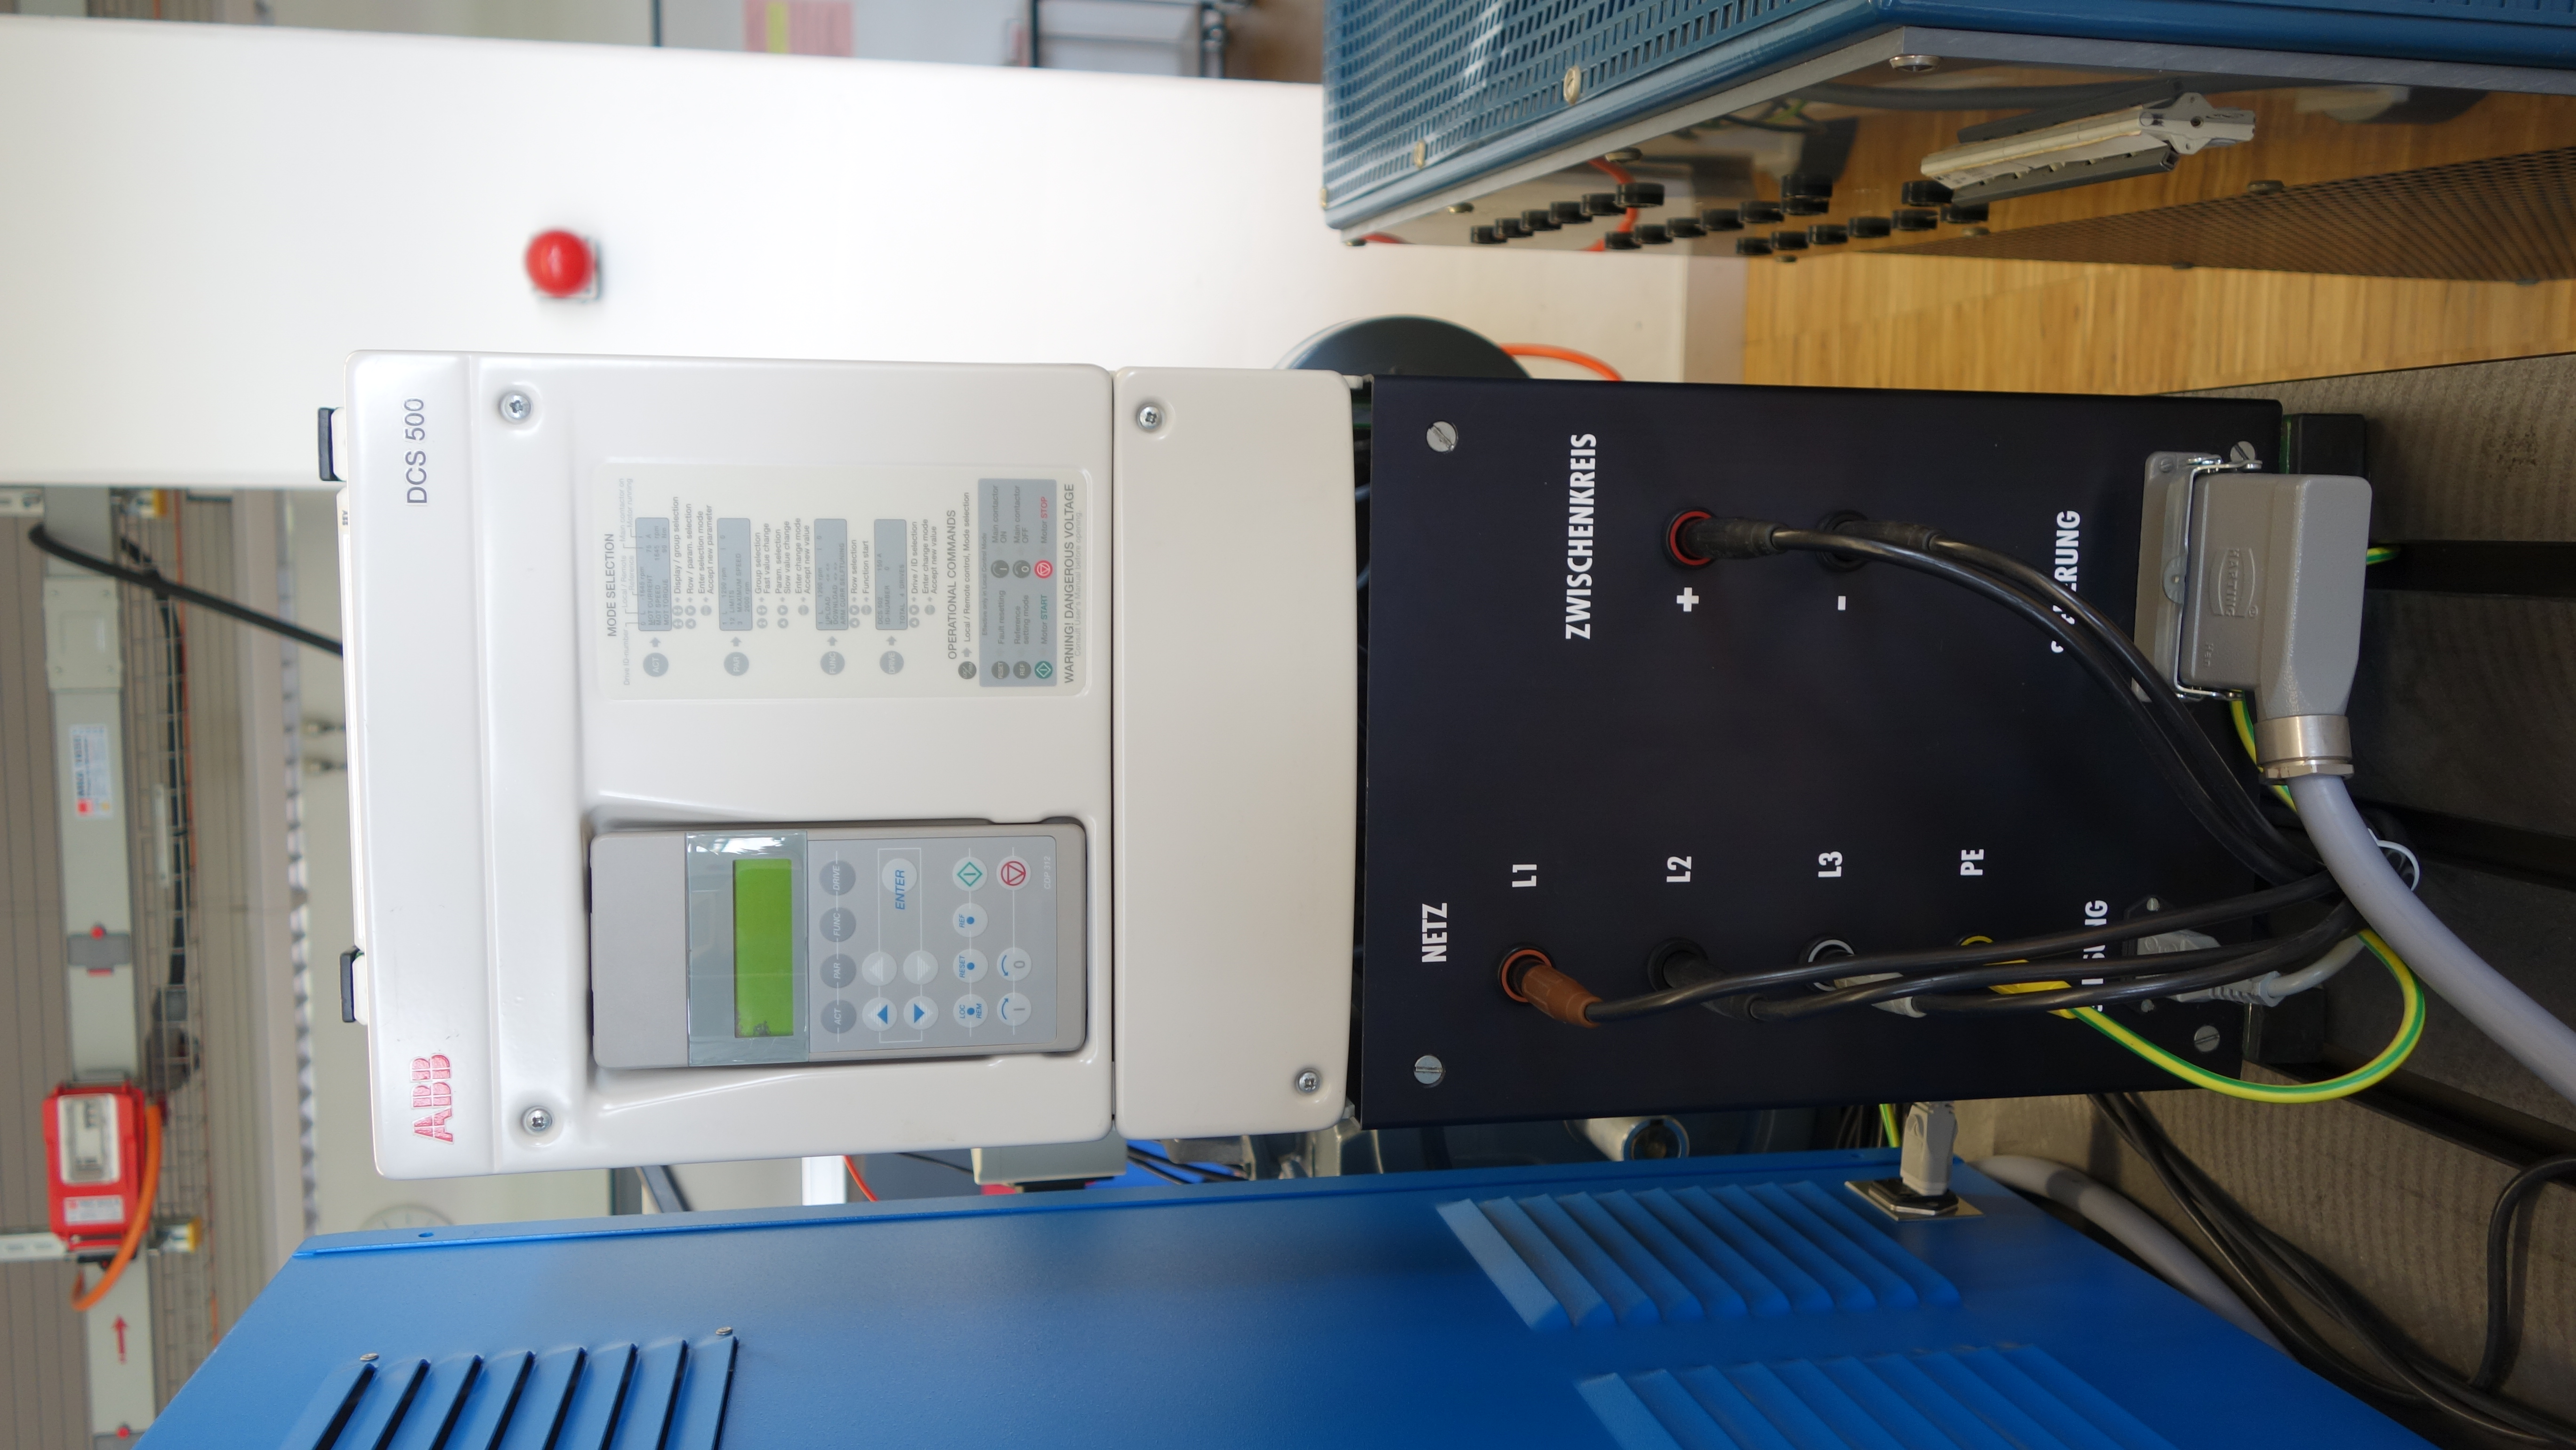
\includegraphics[width=5cm,angle=-90]{images/Gleichrichter.JPG}}
	\caption{Einrichtung}
    \label{fig:einrichtung}
\end{figure}

\clearpage

\chapter{Versuchsaufbau}
\section{Übersichtsschema}
\begin{figure}[h]
	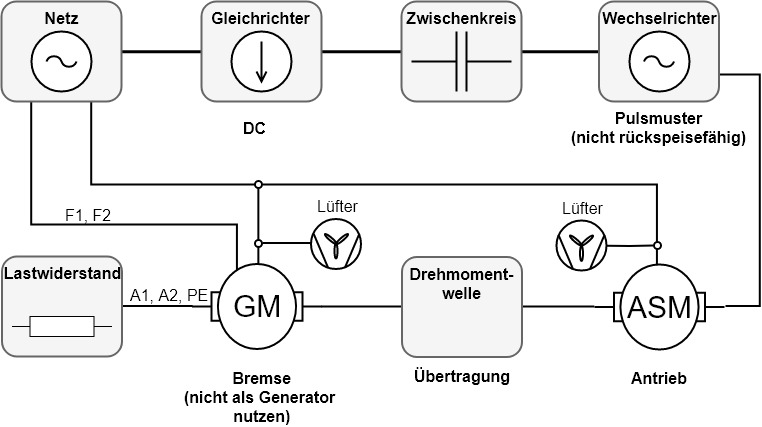
\includegraphics[width=0.9\textwidth]{images/Versuchsaufbau.jpg}
	\caption{Übersichtsschema}
	\label{fig:uebersichtsschema}
\end{figure}
\section{Anmerkungen}
\begin{itemize}
\item Der Frequenzumrichter ist nicht rückspeisefähig. Die GM darf auf keinen Fall als Motor betrieben werden. Die GM darf nicht am Stromrichter angeschlossen werden.
\item Bremsenergie wird über einen Widerstand (81\si{\ohm}  in Wärme  umgewandelt.
\item Lüftungsventiltoren ASM einschalten, besonders bei tiefen Drehzahlen.
\item Leistungsmessgerät PM 3000 über Filter mit Wechselrichter Ausgangsspannung synchronisieren, damit Grundfrequenz bestimmbar.
\end{itemize}

\chapter{Aufgaben}
\minitoc
\minilof
\minilot
%\newpage
\section{Aufgabe 1}
\section{Aufgabe 2}
\section{Optimierte Pulsmuster}

\begin{subequations} \label{eq:equations}
\begin{align}
M*\frac{\pi}{4} &= [1-2*\cos(\alpha_1)+2*\cos(\alpha_2)]
\label{eq:pulsmuster1}\\
Û_v = 0 &= \underbrace{\frac{4}{\pi}}_{test}*\underbrace{\frac{U_{dc}}{2}}_{Zwischenkreis}\frac{1}{\upsilon}[1-2*\cos(\upsilon*\alpha_1)+2*\cos(\upsilon*\alpha_2)]
\label{eq:pulsmuster2}
\end{align}
\end{subequations}


%% Example subequation
%\begin{subequations} \label{eq:equations}
%\begin{align}
%y 	& = a + f(\underbrace{b x}_{\ge 0}) \label{eq:eqsub_1}\\
%z	& = b + a \label{eq:eqsub_2}
%\end{align}
%\end{subequations}

%% Example linear equations
%\begin{align}
%	\begin{array}{*{3}{rc}r}
%	2x & + &  y & + & 3z & = & 10 \\
% 	x & + &  y & + &  z & = &  6 \\
%	 x & + & 3y & + & 2z & = & 13
%	\end{array}
%\end{align}


\begin{align}
\text{Luftwiderstand:} &&
F_{Drag}=F_L=C_W*A*\frac{\rho}{2}*v^2
\label{eq:Luftwiderstand}\\
\text{Barometrische Höhenformel:} &&
p(h_1)=p(h_0)(1-\frac{0.0065*\Delta h}{T(h_0)} )
\label{eq:BarometrischeHoehenformel}\\
\text{Raketengleichung:} &&
m*a=F_{thrust}-F_{drag}-m*g\\
&&
a=\frac{F_{thrust}-F_{drag}-m*g}{m}
\label{eq:Raketengleichung}
\end{align}

\clearpage

\chapter{Titel}
\clearpage

%----- | < Literaturverzeichnis > | -----
%\chapter*{Literatur- und Quellenverzeichnis}
%\renewcommand{\refname}{Quellen-, Literaturverzeichnis}
\bibliographystyle{apacite}
\bibliography{bib/bibliography}
%\bibliographycommon{../common/bib/bibliography}

%---------- | < Anhang > | ----------
\appendix		% Anhang
\chapter{Anhang}

\backmatter		%Ende des Buches, turns off pagenumberin !
\clearpage
\end{document}